\documentclass[tikz]{standalone}
\usepackage{tikz}

\begin{document}
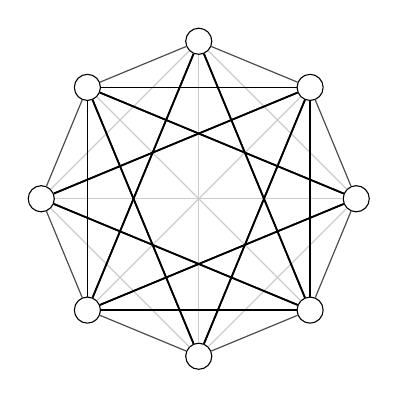
\begin{tikzpicture}
\def \n {8}
\def \radius {2cm}

% draw the edges
\foreach \i [count=\j from 0] in {1,...,\n}
    \node (\i) [circle, draw] at (\j*360/\n:\radius) {};

% complete the graph
\foreach \i in {1,...,\n}
    \foreach \j in {1,...,\i}
        \draw[black!20] (\i) -- (\j);

% draw boundary in a different colour
\pgfmathtruncatemacro{\nn}{\n -1} 
\foreach \i in {1,...,\nn}
    \pgfmathtruncatemacro{\j}{\i +1}
    \draw[black!70] (\i) -- (\j);
\draw[black!70] (\n) -- (1);


% add some symmetries for \n = 8
\foreach \i in {2,4,7}
    \foreach \j in {2,4,7}
        \draw[semithick] (\i) -- (\j);

\foreach \i in {3,6,8}
    \foreach \j in {3,6,8}
        \draw[semithick] (\i) -- (\j);

\foreach \i in {1,4,6}
    \foreach \j in {1,4,6}
        \draw[semithick] (\i) -- (\j);
        
\foreach \i in {2,5,8}
    \foreach \j in {2,5,8}
        \draw[semithick] (\i) -- (\j);


\end{tikzpicture}
\end{document}